% This must be in the first 5 lines to tell arXiv to use pdfLaTeX, which is strongly recommended.
\pdfoutput=1
% In particular, the hyperref package requires pdfLaTeX in order to break URLs across lines.

\documentclass[11pt]{article}

% Remove the "review" option to generate the final version.
\usepackage[review]{ACL2023}

% Standard package includes
\usepackage{times}
\usepackage{latexsym}
\usepackage[capitalize]{cleveref}

% For proper rendering and hyphenation of words containing Latin characters (including in bib files)
\usepackage[T1]{fontenc}
% For Vietnamese characters
% \usepackage[T5]{fontenc}
% See https://www.latex-project.org/help/documentation/encguide.pdf for other character sets

% This assumes your files are encoded as UTF8
\usepackage[utf8]{inputenc}

% This is not strictly necessary, and may be commented out.
% However, it will improve the layout of the manuscript,
% and will typically save some space.
\usepackage{microtype}

% This is also not strictly necessary, and may be commented out.
% However, it will improve the aesthetics of text in
% the typewriter font.
\usepackage{inconsolata}

\usepackage{graphicx}


% If the title and author information does not fit in the area allocated, uncomment the following
%
%\setlength\titlebox{<dim>}
%
% and set <dim> to something 5cm or larger.

\title{Project title}

\author{First Author \\email\And
  Second Author \\email\And
  Third Author \\email}

\begin{document}
\maketitle
\begin{abstract}
This is the abstract.
\end{abstract}

\section{Introduction}

In this Section, describe:
\begin{itemize}
    \item What are you trying to do? Articulate your objectives using absolutely no jargon.
    \item How is it done today, and what are the limits of current practice?
    \item What is new in your approach and why do you think it will be successful?
    \item Who cares? If you are successful, what difference will it make?
\end{itemize}

In this section, you would probably want to reference other papers, use one of the following formats:
\begin{itemize}
    \item In brackets: previous studies~\cite{silberer2014learning} have shown that...
    \item Not in brackets: previously, \citet{silberer2014learning} have shown that...
\end{itemize}

\section{Data}
In this Section, specify the data you used in your experiments. Be sure to include data statistics, is it synthetic/real world, reference the original paper if it wasn't created by you, and more. If you want to use a table (e.g., for data statistics), use the format of \cref{tab:example}. Be sure to locate all tables and figures in the additional page dedicated for this purpose.

\section{Methods}
In this Section, describe the methods used in your experiments. If you trained a model, describe the model architecture, the training method (including loss functions, hyper-parameters choice, etc.) and evaluation method. If you used other procedures such as clustering, describe them here.

\section{Results}
In this Section describe your experimental results. Reference tables and figures if needed, but locate them in the dedicated extra page like \cref{tab:example} and \cref{fig:example}.

\clearpage

% Figures and tables: one page

\begin{table}
\centering
\begin{tabular}{ccc}
\hline
\textbf{Cat} & \textbf{Sample \#} & \textbf{MSL} \\
\hline
Positive & 1200 & 6.3 \\
Negative & 1100 & 9.7 \\
Neutral & 500 &  5.8 \\
Overall & 2800 & 7.55 \\\hline
\end{tabular}
\caption{Example of a table describing data statistics. \emph{Cat} is the category of the sample, \emph{Sample \#} is the number of samples, \emph{MSL} is the mean sentence length for the input sentences.}
\label{tab:example}
\end{table}

\begin{figure}
    \centering
    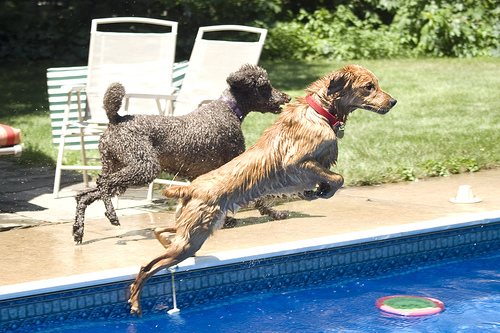
\includegraphics[width=7cm]{dogs.jpg}
    \caption{Example of a figure.}
    \label{fig:example}
\end{figure}

\clearpage

% References

\bibliography{bib}
\bibliographystyle{acl_natbib}

\end{document}
